\section{Modello di sviluppo} \label{section:modello_di_sviluppo}
Il gruppo ha deciso di lavorare secondo il \textbf{modello incrementale} per il \textit{ciclo di vita}\glo{} del software per i seguenti motivi:
\begin{itemize}
  \item Può produrre valore ad ogni incremento, aiutando a fissare meglio i requisiti per gli incrementi successivi;
  \item Ogni incremento riduce il rischio di fallimento;
  \item Le funzionalità principali sono sviluppare nei primi incrementi, rendendole via via più stabili.
\end{itemize}
Nel modello incrementale i requisiti vengono classificati in base alla loro importanza strategica. In questo modo, quelli più importanti vengono 
trattati prima. Questo ne aumenta la chiarezza e la facilità di soddisfazione. I requisiti meno importanti invece vengono soddisfatti in seguito, 
venendo così inseriti in un sistema già stabilizzato.\\
Il metodo di lavoro sarà quindi questo:
\begin{itemize}
  \item In ogni fase di lavoro vengono prefissati degli incrementi che devono essere prodotti entro una scadenza decisa dal gruppo;
  \item Il lavoro viene diviso tra i membri del gruppo;
  \item Al termine del periodo prefissato, una riunione servirà per analizzare il lavoro svolto da ogni membro, riscontrare problemi e difficoltà;
  \item Sarà compito dei \roleVerifier{} controllare il lavoro svolto dagli altri membri del gruppo e sollevare eventuali incongruenze o errori;
  \item Alla fine di questa verifica, seguirà una nuova discussione di gruppo per stabilire se gli obiettivi dell'incremento sono stati soddisfatti.
\end{itemize}

\begin{figure}[H]
	\centering
  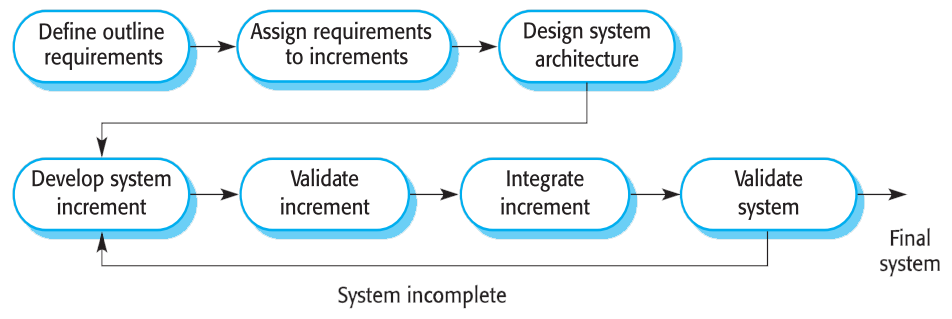
\includegraphics[scale=0.6]{immagini/modello_incrementale.png}
  \caption{Modello incrementale - tratto da: Ian Sommerville, \textit{Software Engineering}, 8th ed.}
\end{figure}
\pagebreak

%%%%%%%%%%%%%%%%%%%%%%%%%%%%%%%%%%%%%%%%%%%%%%%%%%%%%%%%%%%%%%%%%%%%%%%%%%%

\subsection{Incrementi individuati} \label{subsection:incrementi}
In seguito è riportata la tabella con indicati gli incrementi individuati, con il rispettivo obiettivo e i requisiti e casi d'uso ad esso associati. 
I requisiti riportati includono tutti i requisiti figli. Tutti i requisiti non riportati sono da intendersi soddisfatti, in parte, da 
ogni incremento. \\
Ogni requisito e caso d'uso è definito tramite il suo codice identificativo; per maggiori informazioni fare riferimento all'\docNameVersionAdR{}.

\begin{table}[H]
  \centering
  \renewcommand{\arraystretch}{1.8}
  \rowcolors{2}{green!100!black!40}{green!100!black!30}
  \begin{tabular}{c|p{6cm}|c|c}
    \rowcolor[HTML]{125E28}
    \color[HTML]{FFFFFF}\textbf{Incr.}
    & \multicolumn{1}{c}{\color[HTML]{FFFFFF}\textbf{Obiettivo}}
    & \color[HTML]{FFFFFF}\textbf{Requisiti}
    & \color[HTML]{FFFFFF}\textbf{Casi d'uso}\\
    \hline
    & & &
  \end{tabular}
  \caption{Incrementi individuati}
\end{table}